\documentclass[10pt, french]{article}\usepackage[]{graphicx}\usepackage[]{color}
% maxwidth is the original width if it is less than linewidth
% otherwise use linewidth (to make sure the graphics do not exceed the margin)
\makeatletter
\def\maxwidth{ %
  \ifdim\Gin@nat@width>\linewidth
    \linewidth
  \else
    \Gin@nat@width
  \fi
}
\makeatother

\definecolor{fgcolor}{rgb}{0.345, 0.345, 0.345}
\newcommand{\hlnum}[1]{\textcolor[rgb]{0.686,0.059,0.569}{#1}}%
\newcommand{\hlstr}[1]{\textcolor[rgb]{0.192,0.494,0.8}{#1}}%
\newcommand{\hlcom}[1]{\textcolor[rgb]{0.678,0.584,0.686}{\textit{#1}}}%
\newcommand{\hlopt}[1]{\textcolor[rgb]{0,0,0}{#1}}%
\newcommand{\hlstd}[1]{\textcolor[rgb]{0.345,0.345,0.345}{#1}}%
\newcommand{\hlkwa}[1]{\textcolor[rgb]{0.161,0.373,0.58}{\textbf{#1}}}%
\newcommand{\hlkwb}[1]{\textcolor[rgb]{0.69,0.353,0.396}{#1}}%
\newcommand{\hlkwc}[1]{\textcolor[rgb]{0.333,0.667,0.333}{#1}}%
\newcommand{\hlkwd}[1]{\textcolor[rgb]{0.737,0.353,0.396}{\textbf{#1}}}%
\let\hlipl\hlkwb

\usepackage{framed}
\makeatletter
\newenvironment{kframe}{%
 \def\at@end@of@kframe{}%
 \ifinner\ifhmode%
  \def\at@end@of@kframe{\end{minipage}}%
  \begin{minipage}{\columnwidth}%
 \fi\fi%
 \def\FrameCommand##1{\hskip\@totalleftmargin \hskip-\fboxsep
 \colorbox{shadecolor}{##1}\hskip-\fboxsep
     % There is no \\@totalrightmargin, so:
     \hskip-\linewidth \hskip-\@totalleftmargin \hskip\columnwidth}%
 \MakeFramed {\advance\hsize-\width
   \@totalleftmargin\z@ \linewidth\hsize
   \@setminipage}}%
 {\par\unskip\endMakeFramed%
 \at@end@of@kframe}
\makeatother

\definecolor{shadecolor}{rgb}{.97, .97, .97}
\definecolor{messagecolor}{rgb}{0, 0, 0}
\definecolor{warningcolor}{rgb}{1, 0, 1}
\definecolor{errorcolor}{rgb}{1, 0, 0}
\newenvironment{knitrout}{}{} % an empty environment to be redefined in TeX

\usepackage{alltt}
%% -----------------------------
%% Préambule
%% -----------------------------
% !TEX encoding = UTF-8 Unicode
% LaTeX Preamble for all cheatsheets
% Author : Gabriel Crépeault-Cauchon

% HOW-TO : copy-paste this file in the same directory as your .tex file, and add in your preamble the next command right after you have specified your documentclass : 
% \input{preamble-cheatsht.tex}
% ---------------------------------------------
% ---------------------------------------------

% Extra note : this preamble creates document that are meant to be used inside the multicols environment. See the documentation on internet for further information.

%% -----------------------------
%% Encoding packages
%% -----------------------------
\usepackage[utf8]{inputenc}
\usepackage[T1]{fontenc}
\usepackage{babel}
\usepackage{lmodern}

%% -----------------------------
%% Variable definition
%% -----------------------------
\def\auteur{Gabriel Crépeault-Cauchon / Nicholas Langevin}
\def\BackgroundColor{white}

%% -----------------------------
%% Margin and layout
%% -----------------------------
% Determine the margin for cheatsheet
\usepackage[landscape, hmargin=1cm, vmargin=1.7cm]{geometry}
\usepackage{multicol}

% Remove automatic indentation after section/subsection title.
\setlength{\parindent}{0cm}

% Save space in cheatsheet by removing space between align environment and normal text.
\usepackage{etoolbox}
\newcommand{\zerodisplayskips}{%
  \setlength{\abovedisplayskip}{0pt}%
  \setlength{\belowdisplayskip}{0pt}%
  \setlength{\abovedisplayshortskip}{0pt}%
  \setlength{\belowdisplayshortskip}{0pt}}
\appto{\normalsize}{\zerodisplayskips}
\appto{\small}{\zerodisplayskips}
\appto{\footnotesize}{\zerodisplayskips}

%% -----------------------------
%% URL and links
%% -----------------------------
\usepackage{hyperref}
\hypersetup{colorlinks = true, urlcolor = gray!70!white, linkcolor = black}

%% -----------------------------
%% Document policy (uncomment only one)
%% -----------------------------
%	\usepackage{concrete}
	\usepackage{mathpazo}
%	\usepackage{frcursive} %% permet d'écrire en lettres attachées
%	\usepackage{aeguill}
%	\usepackage{mathptmx}
%	\usepackage{fourier} 

%% -----------------------------
%% Math configuration
%% -----------------------------
\usepackage[fleqn]{amsmath}
\usepackage{amsthm,amssymb,latexsym,amsfonts}
\usepackage{empheq}
\usepackage{numprint}
\usepackage{dsfont} % Pour avoir le symbole du domaine Z

% Mathematics shortcuts

\newcommand{\reels}{\mathbb{R}}
\newcommand{\entiers}{\mathbb{Z}}
\newcommand{\naturels}{\mathbb{N}}
\newcommand{\eval}{\biggr \rvert}
\usepackage{cancel}
\newcommand{\derivee}[1]{\frac{\partial}{\partial #1}}
\newcommand{\prob}[1]{\Pr \left( #1 \right)}
\newcommand{\esp}[1]{\mathrm{E} \left[ #1 \right]} % espérance
\newcommand{\variance}[1]{\mathrm{Var} \left( #1   \right)}
\newcommand{\covar}[1]{\mathrm{Cov} \left( #1   \right)}
\newcommand{\laplace}{\mathcal{L}}
\newcommand{\deriv}[2][]{\frac{\partial^{#1}}{\partial #2^{#1}}}
\newcommand{\e}[1]{\mathrm{e}^{#1}}
\newcommand{\te}[1]{\text{exp}\left\{#1\right\}}
\DeclareMathSymbol{\shortminus}{\mathbin}{AMSa}{"39}



% To indicate equation number on a specific line in align environment
\newcommand\numberthis{\addtocounter{equation}{1}\tag{\theequation}}

%
% Actuarial notation packages
%
\usepackage{actuarialsymbol}
\usepackage{actuarialangle}

%
% Matrix notation for math symbols (\bm{•})
%
\usepackage{bm}
% Matrix notation variable (bold style)
\newcommand{\matr}[1]{\mathbf{#1}}



%% -----------------------------
%% tcolorbox configuration
%% -----------------------------
\usepackage[most]{tcolorbox}
\tcbuselibrary{xparse}
\tcbuselibrary{breakable}

%%
%% Coloured box "definition" for definitions
%%
\DeclareTColorBox{definition}{ o }				% #1 parameter
{
	colframe=blue!60!green,colback=blue!5!white, % color of the box
	breakable, 
	pad at break* = 0mm, 						% to split the box
	title = {#1},
	after title = {\large \hfill \faBook},
}
%%
%% Coloured box "definition2" for definitions
%%
\DeclareTColorBox{definitionNOHFILL}{ o }				% #1 parameter
{
	colframe=blue!60!green,colback=blue!5!white, % color of the box
	pad at break* = 0mm, 						% to split the box
	title = {#1},
	before title = {\faBook \quad },
	breakable
}


%%
%% Coloured box "algo" for algorithms
%%
\newtcolorbox{algo}[ 1 ]
{
	colback = blue!5!white,
	colframe = blue!75!black,
	title=#1,
	fonttitle = \bfseries,
	breakable
}
%%
%% Coloured box "conceptgen" for points adding to a concept's deifintion
%%
\newtcolorbox{conceptgen}[ 1 ]
{
	breakable,
	colback = beaublue,
	colframe = airforceblue,
	title=#1,
	fonttitle = \bfseries
}
%%
%% Coloured box "probch3" pour formules relatives au 3ème chapitre de prob
%%
\newtcolorbox{probch3}[ 1 ]
{
	colback = ruddypink,
	colframe = burgundy,
	fonttitle = \bfseries,	
	breakable,
	title=#1
}
%%
%% Coloured box "formula" for formulas
%%
\newtcolorbox{formula}[ 1 ]
{
	colback = green!5!white,
	colframe = green!70!black,
	breakable,
	fonttitle = \bfseries,
	title=#1
}
%%
%% Coloured box "formula" for formulas
%%
\DeclareTColorBox{algo2}{ o }
{
	enhanced,
	title = #1,
	colback=blue!5!white,	
	colbacktitle=blue!75!black,
	fonttitle = \bfseries,
	breakable,
	boxed title style={size=small,colframe=arsenic} ,
	attach boxed title to top center = {yshift=-3mm,yshifttext=-1mm},
}
%%
%% Coloured box "examplebox" for formulas
%%
\newtcolorbox{examplebox}[ 1 ]
{
	colback = lightmauve,
	colframe = antiquefuchsia,
	breakable,
	fonttitle = \bfseries,title=#1
}
%%
%% Coloured box "rappel" pour rappel de formules
%%
\newtcolorbox{rappel}[ 1 ]
{
	colback = ashgrey,
	colframe = arsenic,
	breakable,
	fonttitle = \bfseries,title=#1
}
%%
%% Coloured box "rappel" pour rappel de formules
%%
\DeclareTColorBox{rappel_enhanced}{ o }
{
	enhanced,
	title = #1,
	colback=ashgrey, % color of the box
%	colframe=blue(pigment),
%	colframe=arsenic,	
	colbacktitle=arsenic,
	fonttitle = \bfseries,
	breakable,
	boxed title style={size=small,colframe=arsenic} ,
	attach boxed title to top center = {yshift=-3mm,yshifttext=-1mm},
}
%%
%% Coloured box "notation" for notation and terminology
%%
\DeclareTColorBox{distributions}{ o }			% #1 parameter
{
	enhanced,
	title = #1,
	colback=gray(x11gray), % color of the box
%	colframe=blue(pigment),
	colframe=arsenic,	
	colbacktitle=aurometalsaurus,
	fonttitle = \bfseries,
	boxed title style={size=small,colframe=arsenic} ,
	attach boxed title to top center = {yshift=-3mm,yshifttext=-1mm},
	breakable
%	left=0pt,
%  	right=0pt,
%    box align=center,
%    ams align*
%  	top=-10pt
}

%% -----------------------------
%% Graphics and pictures
%% -----------------------------
\usepackage{graphicx}
\usepackage{pict2e}
\usepackage{tikz}

%% -----------------------------
%% insert pdf pages into document
%% -----------------------------
\usepackage{pdfpages}

%% -----------------------------
%% Color configuration
%% -----------------------------
\usepackage{color, soulutf8, colortbl}


%
%	Colour definitions
%
\definecolor{blue(munsell)}{rgb}{0.0, 0.5, 0.69}
\definecolor{blue(matcha)}{rgb}{0.596, 0.819, 1.00}
\definecolor{blue(munsell)-light}{rgb}{0.5, 0.8, 0.9}
\definecolor{bleudefrance}{rgb}{0.19, 0.55, 0.91}
\definecolor{blizzardblue}{rgb}{0.67, 0.9, 0.93}
\definecolor{bondiblue}{rgb}{0.0, 0.58, 0.71}
\definecolor{blue(pigment)}{rgb}{0.2, 0.2, 0.6}
\definecolor{bluebell}{rgb}{0.64, 0.64, 0.82}
\definecolor{airforceblue}{rgb}{0.36, 0.54, 0.66}
\definecolor{beaublue}{rgb}{0.74, 0.83, 0.9}
\definecolor{cobalt}{rgb}{0.0, 0.28, 0.67}	% nice light blue-ish
\definecolor{blue_rectangle}{RGB}{83, 84, 244}		% ACT-2004
\definecolor{indigo(web)}{rgb}{0.29, 0.0, 0.51}	% purple-ish
\definecolor{antiquefuchsia}{rgb}{0.57, 0.36, 0.51}	%	pastel dark purple ish
\definecolor{darkpastelpurple}{rgb}{0.59, 0.44, 0.84}
\definecolor{gray(x11gray)}{rgb}{0.75, 0.75, 0.75}
\definecolor{aurometalsaurus}{rgb}{0.43, 0.5, 0.5}
\definecolor{ruddypink}{rgb}{0.88, 0.56, 0.59}
\definecolor{pastelred}{rgb}{1.0, 0.41, 0.38}		
\definecolor{lightmauve}{rgb}{0.86, 0.82, 1.0}
\definecolor{azure(colorwheel)}{rgb}{0.0, 0.5, 1.0}
\definecolor{darkgreen}{rgb}{0.0, 0.2, 0.13}			
\definecolor{burntorange}{rgb}{0.8, 0.33, 0.0}		
\definecolor{burntsienna}{rgb}{0.91, 0.45, 0.32}		
\definecolor{ao(english)}{rgb}{0.0, 0.5, 0.0}		% ACT-2003
\definecolor{amber(sae/ece)}{rgb}{1.0, 0.49, 0.0} 	% ACT-2004
\definecolor{green_rectangle}{RGB}{131, 176, 84}		% ACT-2004
\definecolor{red_rectangle}{RGB}{241,112,113}		% ACT-2004
\definecolor{amethyst}{rgb}{0.6, 0.4, 0.8}
\definecolor{amethyst-light}{rgb}{0.6, 0.4, 0.8}
\definecolor{ashgrey}{rgb}{0.7, 0.75, 0.71}			% dark grey-black-ish
\definecolor{arsenic}{rgb}{0.23, 0.27, 0.29}			% light green-beige-ish gray
\definecolor{amaranth}{rgb}{0.9, 0.17, 0.31}
\definecolor{brickred}{rgb}{0.8, 0.25, 0.33}
\definecolor{pastelred}{rgb}{1.0, 0.41, 0.38}

%
% Useful shortcuts for coloured text
%
\newcommand{\orange}{\textcolor{orange}}
\newcommand{\red}{\textcolor{red}}
\newcommand{\cyan}{\textcolor{cyan}}
\newcommand{\blue}{\textcolor{blue}}
\newcommand{\green}{\textcolor{green}}
\newcommand{\purple}{\textcolor{magenta}}
\newcommand{\yellow}{\textcolor{yellow}}

%% -----------------------------
%% Enumerate environment configuration
%% -----------------------------
%
% Custum enumerate & itemize Package
%
\usepackage{enumitem}
%
% French Setup for itemize function
%
\frenchbsetup{StandardItemLabels=true}
%
% Change default label for itemize
%
\renewcommand{\labelitemi}{\faAngleRight}


%% -----------------------------
%% Tabular column type configuration
%% -----------------------------
\newcolumntype{C}{>{$}c<{$}} % math-mode version of "l" column type
\newcolumntype{L}{>{$}l<{$}} % math-mode version of "l" column type
\newcolumntype{R}{>{$}r<{$}} % math-mode version of "l" column type
\newcolumntype{f}{>{\columncolor{green!20!white}}p{1cm}}
\newcolumntype{g}{>{\columncolor{green!40!white}}m{1.2cm}}
\newcolumntype{a}{>{\columncolor{red!20!white}$}p{2cm}<{$}}	% ACT-2005
% configuration to force a line break within a single cell
\usepackage{makecell}


%% -----------------------------
%% Fontawesome for special symbols
%% -----------------------------
\usepackage{fontawesome}

%% -----------------------------
%% Section Font customization
%% -----------------------------
\usepackage{sectsty}
\sectionfont{\color{\SectionColor}}
\subsectionfont{\color{\SubSectionColor}}

%% -----------------------------
%% Footer/Header Customization
%% -----------------------------
\usepackage{lastpage}
\usepackage{fancyhdr}
\pagestyle{fancy}

%
% Header
%
\fancyhead{} 	% Reset
\fancyhead[L]{Aide-mémoire pour~ \cours ~(\textbf{\sigle})}
\fancyhead[R]{\auteur}

%
% Footer
%
\fancyfoot{}		% Reset
\fancyfoot[R]{\thepage ~de~ \pageref{LastPage}}
\fancyfoot[L]{\href{https://github.com/ressources-act/Guide_de_survie_en_actuariat}{\faGithub \ ressources-act/Guide de survie en actuariat}}
%
% Page background color
%
\pagecolor{\BackgroundColor}




%% END OF PREAMBLE
% ---------------------------------------------
% ---------------------------------------------
%% -----------------------------
%% Variable definition
%% -----------------------------
\def\cours{Apprentissage statistique en actuariat}
\def\sigle{ACT-3114}
%% -----------------------------
%% Colour setup for sections
%% -----------------------------
\def\SectionColor{green!50!black}
\def\SubSectionColor{green!20!black}
\def\SubSubSectionColor{burntsienna}

%	"to-do" list
\newlist{todolist}{itemize}{2}
\setlist[todolist]{label=$\square$}
%%%

\usetikzlibrary{fit, matrix}
\definecolor{ballblue}{rgb}{0.13, 0.67, 0.8}
\definecolor{darkgreen}{rgb}{0.0, 0.2, 0.13}
\definecolor{rstudioblue}{RGB}{247, 247, 247}
\lstset{language=R,
    basicstyle=\small\ttfamily,
    stringstyle=\color{darkgreen},
    otherkeywords={0,1,2,3,4,5,6,7,8,9},
    morekeywords={TRUE,FALSE},
    deletekeywords={data,frame,length,as,character},
    keywordstyle=\color{blue},
    commentstyle=\color{darkgreen},
}




\setcounter{secnumdepth}{0}


%% -----------------------------
%% Début du document
%% -----------------------------
\IfFileExists{upquote.sty}{\usepackage{upquote}}{}
\begin{document}
\begin{center}
	\textsc{\Large Contributeurs}\\[0.5cm] 
\end{center}
\begin{contrib}{ACT-3114\: Apprentissage statistique en actuariat}
\begin{description}
	\item[aut.] Alec James van Rassel
	\item[ctb.]	Alexis Picard
	\item[ctb.]	Gabriel Lord
	\item[src.] Marie-Pier Côté
\end{description}
\end{contrib}

\newpage


\section{Fonctions \texttt{R}}

\begin{center}
	\textbf{Dupliqués et niveaux}
\end{center}
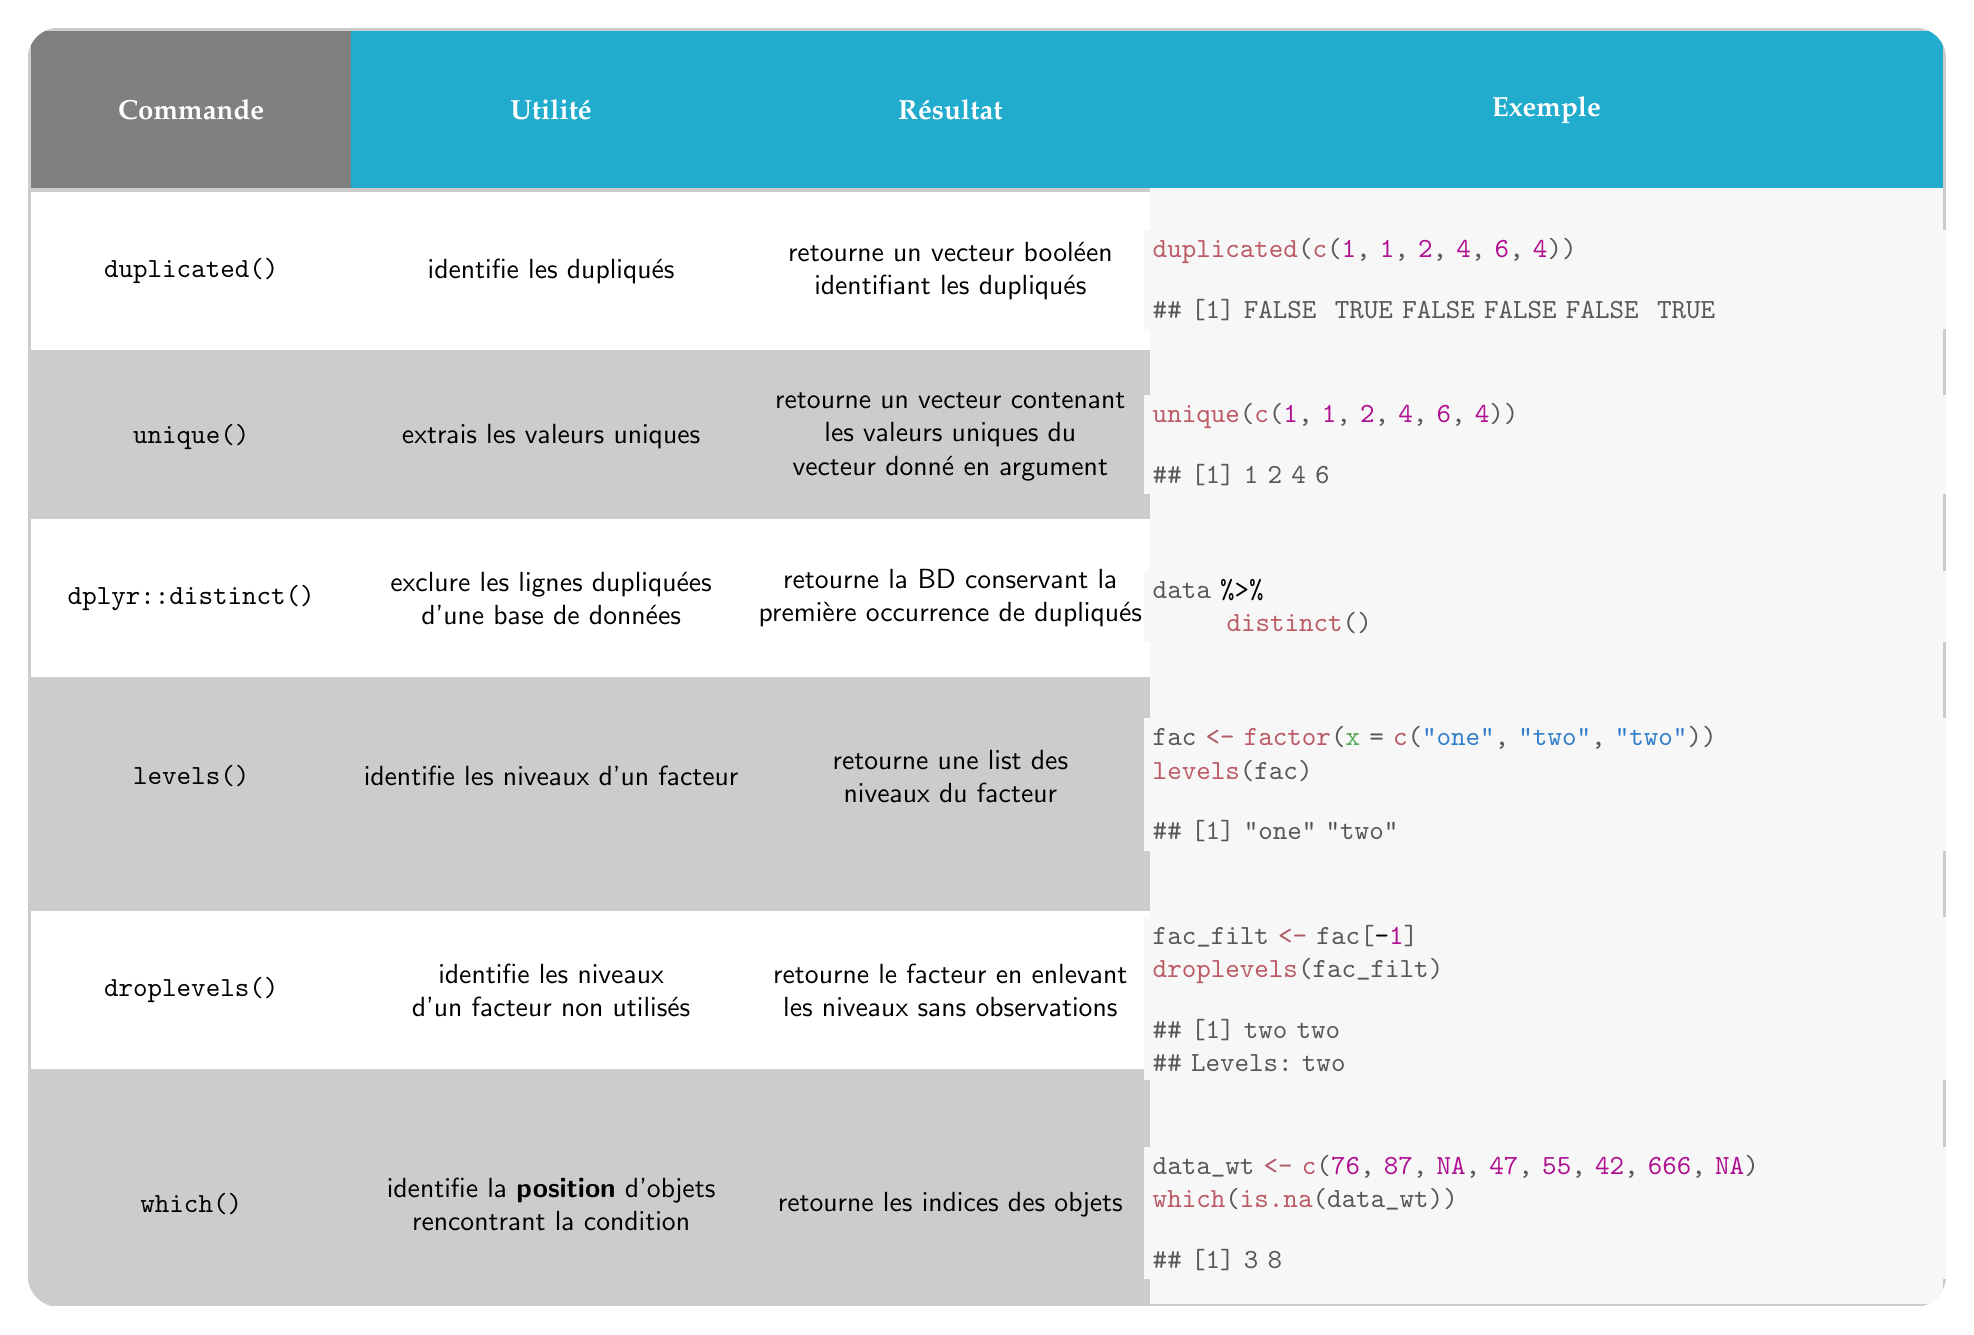
\begin{tikzpicture}
\clip node (m) [
	matrix,
	matrix of nodes,
	fill = black!20, % alternating rows color
	inner sep = 1pt, % width of exterior line
	nodes in empty cells,
	nodes = {
		minimum height = 2cm,
		minimum width = 2.6cm,
		anchor = center,
		outer sep = 0,
		font = \sffamily
	},
	row 1/.style = {
		nodes = {
			fill = ballblue,  % header colour
			text = white,
			font = \bfseries
		}
	},
	column 1/.style = {
		text width = 4cm, 
		align = center,
		nodes = {
			font = \bfseries
		},
		every even row/.style = {
			nodes = {
				fill = white
			}
		}
	},
	column 2/.style = {
		text width = 5cm,
		align = center,
		every even row/.style = {nodes = {fill = white}},
	},
	column 3/.style = {
		text width = 5cm,
		align = center,
		every even row/.style = {nodes = {fill = white}},
	},
	column 4/.style = {
		text width = 10cm,
		align = center,
		nodes = {fill = rstudioblue}
	},
	row 1 column 1/.style = {nodes = {fill = gray}},
	prefix after command = {
		[rounded corners = 4mm] (m.north east) rectangle (m.south west)
	}
] {
	Commande	&	Utilité	&	Résultat	&	Exemple \\
	\texttt{duplicated()}	&	identifie les dupliqués	&	retourne un vecteur booléen identifiant les dupliqués	&	
\begin{knitrout}
\definecolor{shadecolor}{rgb}{0.969, 0.969, 0.969}\color{fgcolor}\begin{kframe}
\begin{alltt}
\hlkwd{duplicated}\hlstd{(}\hlkwd{c}\hlstd{(}\hlnum{1}\hlstd{,} \hlnum{1}\hlstd{,} \hlnum{2}\hlstd{,} \hlnum{4}\hlstd{,} \hlnum{6}\hlstd{,} \hlnum{4}\hlstd{))}
\end{alltt}
\begin{verbatim}
## [1] FALSE  TRUE FALSE FALSE FALSE  TRUE
\end{verbatim}
\end{kframe}
\end{knitrout}
	\\
	\texttt{unique()}	&	extrais les valeurs uniques	&	retourne un vecteur contenant les valeurs uniques du vecteur donné en argument	&
\begin{knitrout}
\definecolor{shadecolor}{rgb}{0.969, 0.969, 0.969}\color{fgcolor}\begin{kframe}
\begin{alltt}
\hlkwd{unique}\hlstd{(}\hlkwd{c}\hlstd{(}\hlnum{1}\hlstd{,} \hlnum{1}\hlstd{,} \hlnum{2}\hlstd{,} \hlnum{4}\hlstd{,} \hlnum{6}\hlstd{,} \hlnum{4}\hlstd{))}
\end{alltt}
\begin{verbatim}
## [1] 1 2 4 6
\end{verbatim}
\end{kframe}
\end{knitrout}
	\\
	\texttt{dplyr::distinct()}	&	exclure les lignes dupliquées d'une base de données	&	retourne la BD conservant la première occurrence de dupliqués	&	
\begin{knitrout}
\definecolor{shadecolor}{rgb}{0.969, 0.969, 0.969}\color{fgcolor}\begin{kframe}
\begin{alltt}
\hlstd{data} \hlopt
        \hlkwd{distinct}\hlstd{()}
\end{alltt}
\end{kframe}
\end{knitrout}
	\\
	\texttt{levels()}	&	identifie les niveaux d'un facteur	&	retourne une list des niveaux du facteur	&	
\begin{knitrout}
\definecolor{shadecolor}{rgb}{0.969, 0.969, 0.969}\color{fgcolor}\begin{kframe}
\begin{alltt}
\hlstd{fac} \hlkwb{<-} \hlkwd{factor}\hlstd{(}\hlkwc{x} \hlstd{=} \hlkwd{c}\hlstd{(}\hlstr{"one"}\hlstd{,} \hlstr{"two"}\hlstd{,} \hlstr{"two"}\hlstd{))}
\hlkwd{levels}\hlstd{(fac)}
\end{alltt}
\begin{verbatim}
## [1] "one" "two"
\end{verbatim}
\end{kframe}
\end{knitrout}
	\\
	\texttt{droplevels()}	&	identifie les niveaux d'un facteur non utilisés	&	retourne le facteur en enlevant les niveaux sans observations	&	
\begin{knitrout}
\definecolor{shadecolor}{rgb}{0.969, 0.969, 0.969}\color{fgcolor}\begin{kframe}
\begin{alltt}
\hlstd{fac_filt} \hlkwb{<-} \hlstd{fac[}\hlopt{-}\hlnum{1}\hlstd{]}
\hlkwd{droplevels}\hlstd{(fac_filt)}
\end{alltt}
\begin{verbatim}
## [1] two two
## Levels: two
\end{verbatim}
\end{kframe}
\end{knitrout}
	\\
	\texttt{which()}		&	identifie la \textbf{position} d'objets rencontrant la condition
&	retourne les indices des objets	&	
\begin{knitrout}
\definecolor{shadecolor}{rgb}{0.969, 0.969, 0.969}\color{fgcolor}\begin{kframe}
\begin{alltt}
\hlstd{data_wt} \hlkwb{<-} \hlkwd{c}\hlstd{(}\hlnum{76}\hlstd{,} \hlnum{87}\hlstd{,} \hlnum{NA}\hlstd{,} \hlnum{47}\hlstd{,} \hlnum{55}\hlstd{,} \hlnum{42}\hlstd{,} \hlnum{666}\hlstd{,} \hlnum{NA}\hlstd{)}
\hlkwd{which}\hlstd{(}\hlkwd{is.na}\hlstd{(data_wt))}
\end{alltt}
\begin{verbatim}
## [1] 3 8
\end{verbatim}
\end{kframe}
\end{knitrout}
	\\
};
\end{tikzpicture}

\begin{center}
	\textbf{Agrégation}
\end{center}
\begin{description}
	\item[\texttt{table()} et \texttt{prop.table()}]	Retourne un tableau de fréquence et de proportion. \\
	À 2 dimensions, il faut s'assurer d'avoir les mêmes dimensions pour les 2 vecteurs. \\
	À 3 dimensions, la fonction retourne un tableau par niveau du troisième argument.\\
	\texttt{prop.table()} s'enchaîne à une table et ne pas être utilisé directement.\\
	L'argument \texttt{margin} spécifie la dimension sur laquelle sommer (1 pour les rangées, 2 pour les colonnes).
\begin{knitrout}
\definecolor{shadecolor}{rgb}{0.969, 0.969, 0.969}\color{fgcolor}\begin{kframe}
\begin{alltt}
\hlstd{facto} \hlkwb{<-} \hlkwd{factor}\hlstd{(}\hlkwc{x} \hlstd{=} \hlkwd{c}\hlstd{(}\hlstr{"deux"}\hlstd{,} \hlstr{"two"}\hlstd{,} \hlstr{"one"}\hlstd{,} \hlstr{"one"}\hlstd{,} \hlstr{"un"}\hlstd{,} \hlstr{"deux"}\hlstd{))}
\hlkwd{table}\hlstd{(facto)}
\end{alltt}
\begin{verbatim}
## facto
## deux  one  two   un 
##    2    2    1    1
\end{verbatim}
\begin{alltt}
\hlstd{age} \hlkwb{<-} \hlkwd{c}\hlstd{(}\hlnum{18}\hlstd{,} \hlnum{20}\hlstd{,} \hlnum{19}\hlstd{,} \hlnum{18}\hlstd{,} \hlnum{20}\hlstd{)}
\hlstd{weight} \hlkwb{<-} \hlkwd{c}\hlstd{(}\hlnum{200}\hlstd{,} \hlnum{150}\hlstd{,} \hlnum{175}\hlstd{,} \hlnum{190}\hlstd{,} \hlnum{220}\hlstd{)}
\hlkwd{table}\hlstd{(age, weight)}
\end{alltt}
\begin{verbatim}
##     weight
## age  150 175 190 200 220
##   18   0   0   1   1   0
##   19   0   1   0   0   0
##   20   1   0   0   0   1
\end{verbatim}
\begin{alltt}
\hlkwd{table}\hlstd{(age, weight)} \hlopt
    \hlkwd{prop.table}\hlstd{(}\hlkwc{margin} \hlstd{=} \hlnum{1}\hlstd{)}
\end{alltt}
\begin{verbatim}
##     weight
## age  150 175 190 200 220
##   18 0.0 0.0 0.5 0.5 0.0
##   19 0.0 1.0 0.0 0.0 0.0
##   20 0.5 0.0 0.0 0.0 0.5
\end{verbatim}
\end{kframe}
\end{knitrout}
	\item[\texttt{aggregate()}]	Calcule une fonction par groupe pour une base de données.\\
		Il faut faire attention à la fonction donnée en argument. Si l’on veut calculer une moyenne et la BD contient des facteurs, la fonction retourne \texttt{NA} pour cette colonne avec un message d'erreur.\\
		Il faut donner l'argument à \texttt{by} en forme de liste même si nous n'avons qu'une seule variable par laquelle grouper.
\begin{knitrout}
\definecolor{shadecolor}{rgb}{0.969, 0.969, 0.969}\color{fgcolor}\begin{kframe}
\begin{alltt}
\hlstd{BD} \hlkwb{<-} \hlkwd{data.frame}\hlstd{(}\hlkwc{age} \hlstd{=} \hlkwd{c}\hlstd{(}\hlnum{18}\hlstd{,} \hlnum{20}\hlstd{,} \hlnum{19}\hlstd{,} \hlnum{18}\hlstd{,} \hlnum{20}\hlstd{),}
                 \hlkwc{weight} \hlstd{=} \hlkwd{c}\hlstd{(}\hlnum{200}\hlstd{,} \hlnum{150}\hlstd{,} \hlnum{175}\hlstd{,} \hlnum{190}\hlstd{,} \hlnum{220}\hlstd{))}
\hlstd{sex} \hlkwb{<-} \hlkwd{factor}\hlstd{(}\hlkwd{c}\hlstd{(}\hlstr{"F"}\hlstd{,} \hlstr{"F"}\hlstd{,} \hlstr{"H"}\hlstd{,} \hlstr{"F"}\hlstd{,} \hlstr{"H"}\hlstd{))}
\hlstd{student} \hlkwb{<-} \hlkwd{as.factor}\hlstd{(}\hlkwd{c}\hlstd{(T, F, T, T, F))}
\hlkwd{aggregate}\hlstd{(}\hlkwc{x} \hlstd{= BD,} \hlkwc{by} \hlstd{=} \hlkwd{list}\hlstd{(sex),} \hlkwc{FUN} \hlstd{= median)}
\end{alltt}
\begin{verbatim}
##   Group.1  age weight
## 1       F 18.0  190.0
## 2       H 19.5  197.5
\end{verbatim}
\begin{alltt}
\hlkwd{aggregate}\hlstd{(}\hlkwc{x} \hlstd{= BD,} \hlkwc{by} \hlstd{=} \hlkwd{list}\hlstd{(sex, student),} \hlkwc{FUN} \hlstd{= median)}
\end{alltt}
\begin{verbatim}
##   Group.1 Group.2 age weight
## 1       F   FALSE  20    150
## 2       H   FALSE  20    220
## 3       F    TRUE  18    195
## 4       H    TRUE  19    175
\end{verbatim}
\end{kframe}
\end{knitrout}
\end{description}

\begin{center}
	\textbf{Modifications de variables}
\end{center}
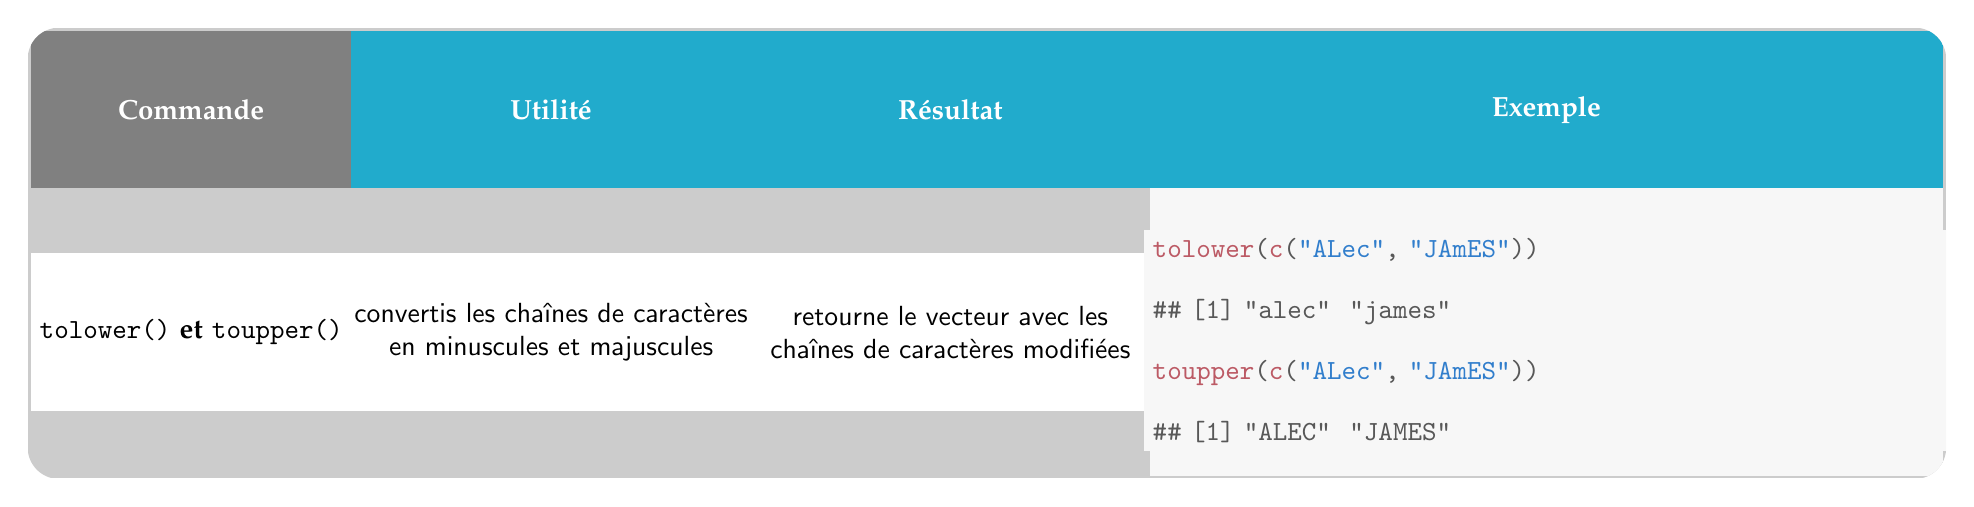
\begin{tikzpicture}
\clip node (m) [
	matrix,
	matrix of nodes,
	fill = black!20, % alternating rows color
	inner sep = 1pt, % width of exterior line
	nodes in empty cells,
	nodes = {
		minimum height = 2cm,
		minimum width = 2.6cm,
		anchor = center,
		outer sep = 0,
		font = \sffamily
	},
	row 1/.style = {
		nodes = {
			fill = ballblue,  % header colour
			text = white,
			font = \bfseries
		}
	},
	column 1/.style = {
		text width = 4cm, 
		align = center,
		nodes = {
			font = \bfseries
		},
		every even row/.style = {
			nodes = {
				fill = white
			}
		}
	},
	column 2/.style = {
		text width = 5cm,
		align = center,
		every even row/.style = {nodes = {fill = white}},
	},
	column 3/.style = {
		text width = 5cm,
		align = center,
		every even row/.style = {nodes = {fill = white}},
	},
	column 4/.style = {
		text width = 10cm,
		align = center,
		nodes = {fill = rstudioblue}
	},
	row 1 column 1/.style = {nodes = {fill = gray}},
	prefix after command = {
		[rounded corners = 4mm] (m.north east) rectangle (m.south west)
	}
] {
	Commande	&	Utilité	&	Résultat	&	Exemple \\
	\texttt{tolower()} et \texttt{toupper()}	&	convertis les chaînes de caractères en minuscules et majuscules	&	retourne le vecteur avec les chaînes de caractères modifiées	&	
\begin{knitrout}
\definecolor{shadecolor}{rgb}{0.969, 0.969, 0.969}\color{fgcolor}\begin{kframe}
\begin{alltt}
\hlkwd{tolower}\hlstd{(}\hlkwd{c}\hlstd{(}\hlstr{"ALec"}\hlstd{,} \hlstr{"JAmES"}\hlstd{))}
\end{alltt}
\begin{verbatim}
## [1] "alec"  "james"
\end{verbatim}
\begin{alltt}
\hlkwd{toupper}\hlstd{(}\hlkwd{c}\hlstd{(}\hlstr{"ALec"}\hlstd{,} \hlstr{"JAmES"}\hlstd{))}
\end{alltt}
\begin{verbatim}
## [1] "ALEC"  "JAMES"
\end{verbatim}
\end{kframe}
\end{knitrout}
	\\
};
\end{tikzpicture}

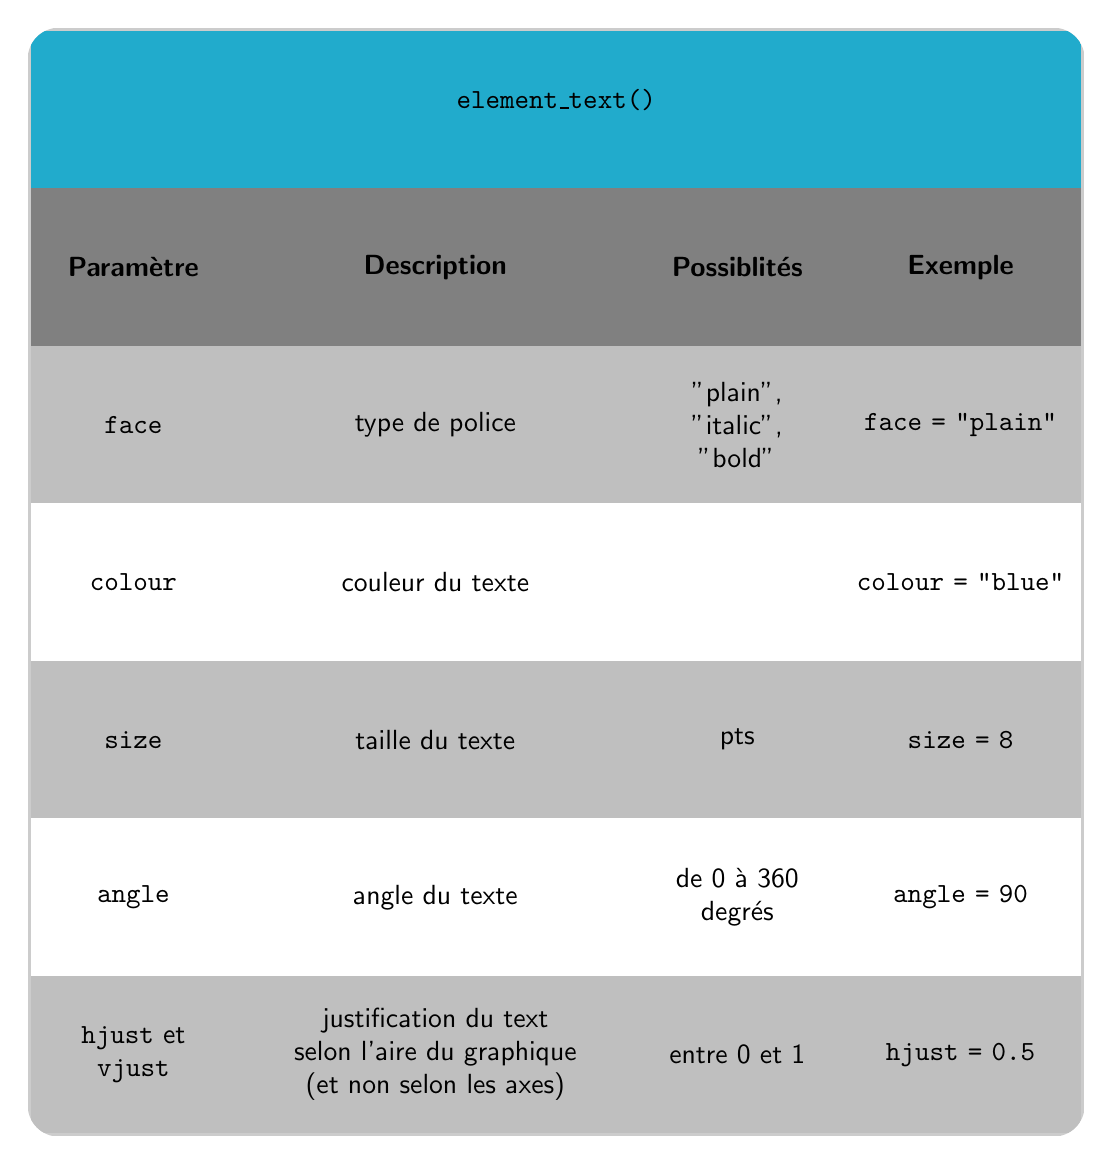
\begin{tikzpicture}
\clip node (m) [
	matrix,
	matrix of nodes,
	fill = black!20, % alternating rows color
	inner sep = 1pt, % width of exterior line
	nodes in empty cells,
	nodes = {
		minimum height = 2cm,
		minimum width = 2.6cm,
		anchor = center,
		outer sep = 0,
		font = \sffamily
	},
	row 1/.style = {
		nodes = {
			fill = ballblue,  % header colour
			text = white,
			font = \bfseries
		}
	},
	column 1/.style = {
		text width = 2cm, 
		align = center,
		nodes = {
			fill = lightgray
		},
		every even row/.style = {
			nodes = {
				fill = white
			}
		}
	},
	column 2/.style = {
		text width = 5cm, 
		align = center,
		nodes = {
			fill = lightgray
		},
		every even row/.style = {
			nodes = {
				fill = white
			}
		}
	},
	column 3/.style = {
		text width = 2cm, 
		align = center,
		nodes = {
			fill = lightgray
		},
		every even row/.style = {
			nodes = {
				fill = white
			}
		}
	},
	column 4/.style = {
		text width = 3cm, 
		align = center,
		nodes = {
			fill = lightgray
		},
		every even row/.style = {
			nodes = {
				fill = white
			}
		}
	},
	row 2 column 1/.style = {nodes = {fill = gray}},
	row 2 column 2/.style = {nodes = {fill = gray}},
	row 2 column 3/.style = {nodes = {fill = gray}},
	row 2 column 4/.style = {nodes = {fill = gray}},
	prefix after command = {
		[rounded corners = 4mm] (m.north east) rectangle (m.south west)
	}
] {
			&			&			&			\\
	\textbf{Paramètre}	&	\textbf{Description}	&	\textbf{Possiblités}	&	\textbf{Exemple} \\
	\texttt{face	}	&	type de police	&	"plain", "italic", "bold"	&	 \texttt{face = "plain"}	\\
	\texttt{colour}	&	couleur du texte	&		&	\texttt{colour = "blue"}	 \\
	\texttt{size}	&	taille du texte&		pts	&	\texttt{size = 8}	 \\
	\texttt{angle}	&	angle du texte	&	de 0 à 360 degrés	&	\texttt{angle = 90}	 \\
	\texttt{hjust} et \texttt{vjust}	&	justification du text selon l'aire du graphique (et non selon les axes) &	entre 0 et 1	&	\texttt{hjust = 0.5}	 \\
};
    \node[fit=(m-1-1)(m-1-4)]{\texttt{element\_text()}\addcontentsline{toc}{subsection}{ggplot2}};
\end{tikzpicture}


\section{Fonctions \texttt{R} pour l'ajustement de modèles}

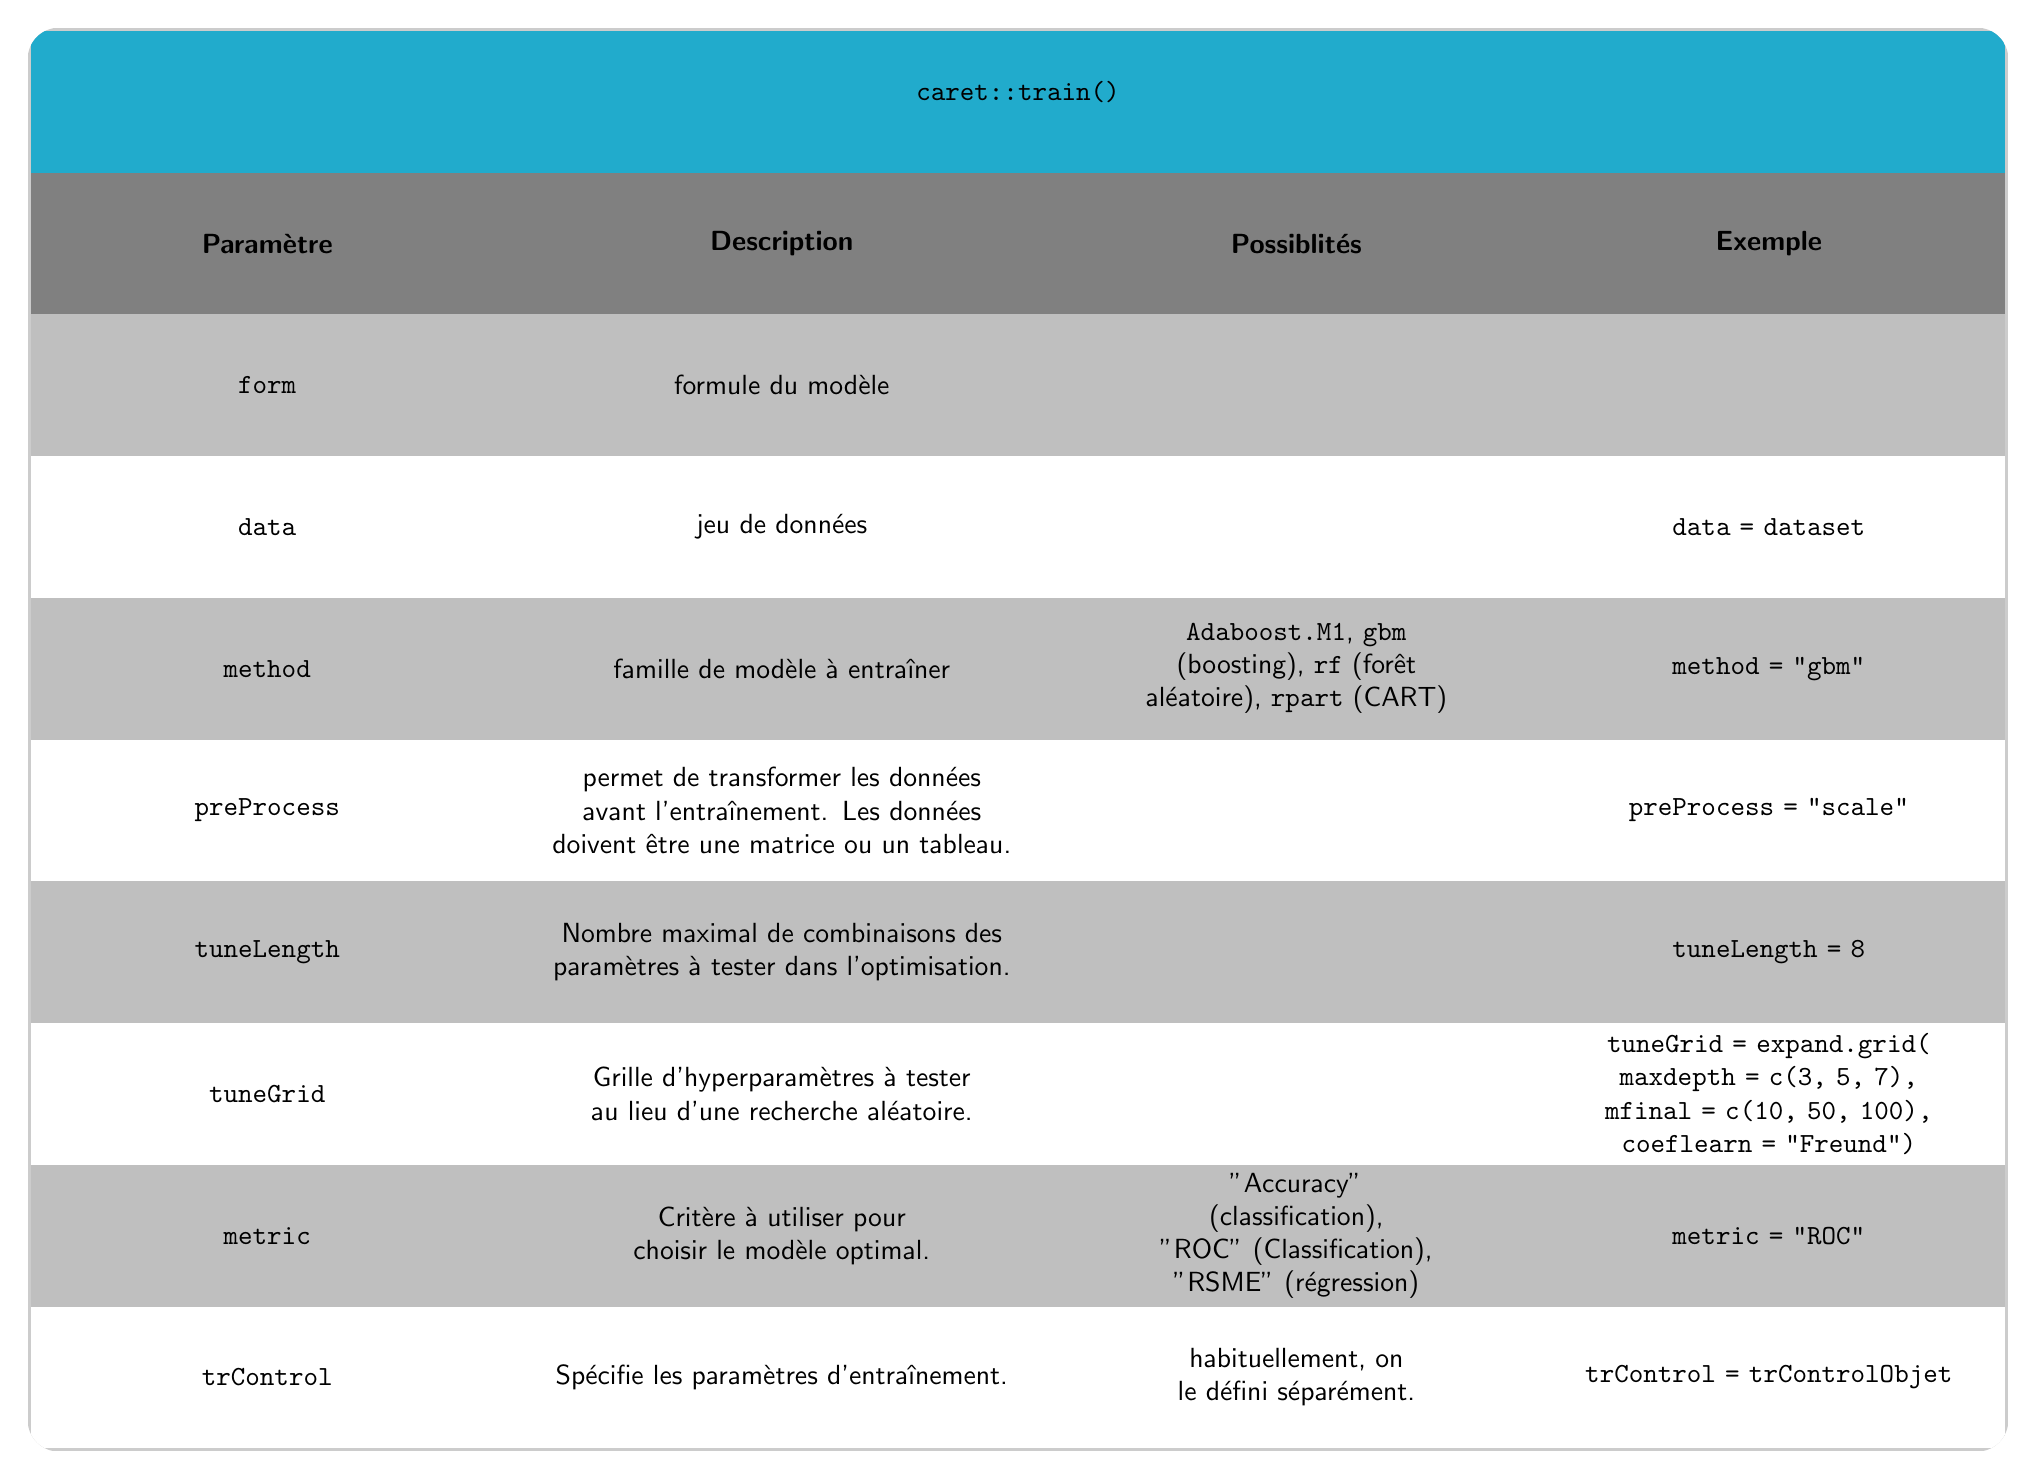
\begin{tikzpicture}
\clip node (m) [
	matrix,
	matrix of nodes,
	fill = black!20, % alternating rows color
	inner sep = 1pt, % width of exterior line
	nodes in empty cells,
	nodes = {
		minimum height = 1.8cm,
		minimum width = 6cm,
		anchor = center,
		outer sep = 0,
		font = \sffamily
	},
	row 1/.style = {
		nodes = {
			fill = ballblue,  % header colour
			text = white,
			font = \bfseries
		}
	},
	column 1/.style = {
		text width = 3cm, 
		align = center,
		nodes = {
			fill = lightgray
		},
		every even row/.style = {
			nodes = {
				fill = white
			}
		}
	},
	column 2/.style = {
		text width = 7cm, 
		align = center,
		nodes = {
			fill = lightgray
		},
		every even row/.style = {
			nodes = {
				fill = white
			}
		}
	},
	column 3/.style = {
		text width = 4cm, 
		align = center,
		nodes = {
			fill = lightgray
		},
		every even row/.style = {
			nodes = {
				fill = white
			}
		}
	},
	column 4/.style = {
		text width = 5cm, 
		align = center,
		nodes = {
			fill = lightgray
		},
		every even row/.style = {
			nodes = {
				fill = white
			}
		}
	},
	row 2 column 1/.style = {nodes = {fill = gray}},
	row 2 column 2/.style = {nodes = {fill = gray}},
	row 2 column 3/.style = {nodes = {fill = gray}},
	row 2 column 4/.style = {nodes = {fill = gray}},
	prefix after command = {
		[rounded corners = 4mm] (m.north east) rectangle (m.south west)
	}
] {
			&			&			&			\\
	\textbf{Paramètre}	&	\textbf{Description}	&	\textbf{Possiblités}	&	\textbf{Exemple} \\
	\texttt{form	}	&	formule du modèle	&	 	&	 	\\
	\texttt{data}	&	jeu de données	&		&	\texttt{data = dataset}	 \\
	\texttt{method}	&	famille de modèle à entraîner	&	\texttt{Adaboost.M1}, \texttt{gbm} (boosting), \texttt{rf} (forêt aléatoire), \texttt{rpart} (CART)	&	\texttt{method = "gbm"}	 \\
	\texttt{preProcess}	&	permet de transformer les données avant l'entraînement. Les données doivent être une matrice ou un tableau.	&		&	\texttt{preProcess = "scale"}	 \\
	\texttt{tuneLength}	&	Nombre maximal de combinaisons des paramètres à tester dans l'optimisation.	&		&	\texttt{tuneLength = 8}	 \\
	\texttt{tuneGrid}	&	Grille d'hyperparamètres à tester au lieu d'une recherche aléatoire.	&		&	
		\texttt{tuneGrid = expand.grid(
		maxdepth = c(3, 5, 7),  
		mfinal = c(10, 50, 100),
		coeflearn = "Freund")}	 \\
	\texttt{metric}	&	Critère à utiliser pour choisir le modèle optimal.	&	"Accuracy" (classification), "ROC" (Classification), "RSME" (régression)	&	\texttt{metric = "ROC"}	 \\
	\texttt{trControl}	&	Spécifie les paramètres d'entraînement.	&	habituellement, on le défini séparément.	&	\texttt{trControl = trControlObjet}	 \\
};
    \node[fit=(m-1-1)(m-1-4)]{\texttt{caret::train()}\addcontentsline{toc}{subsection}{Entraînement de modèles}};
\end{tikzpicture}

\pagebreak

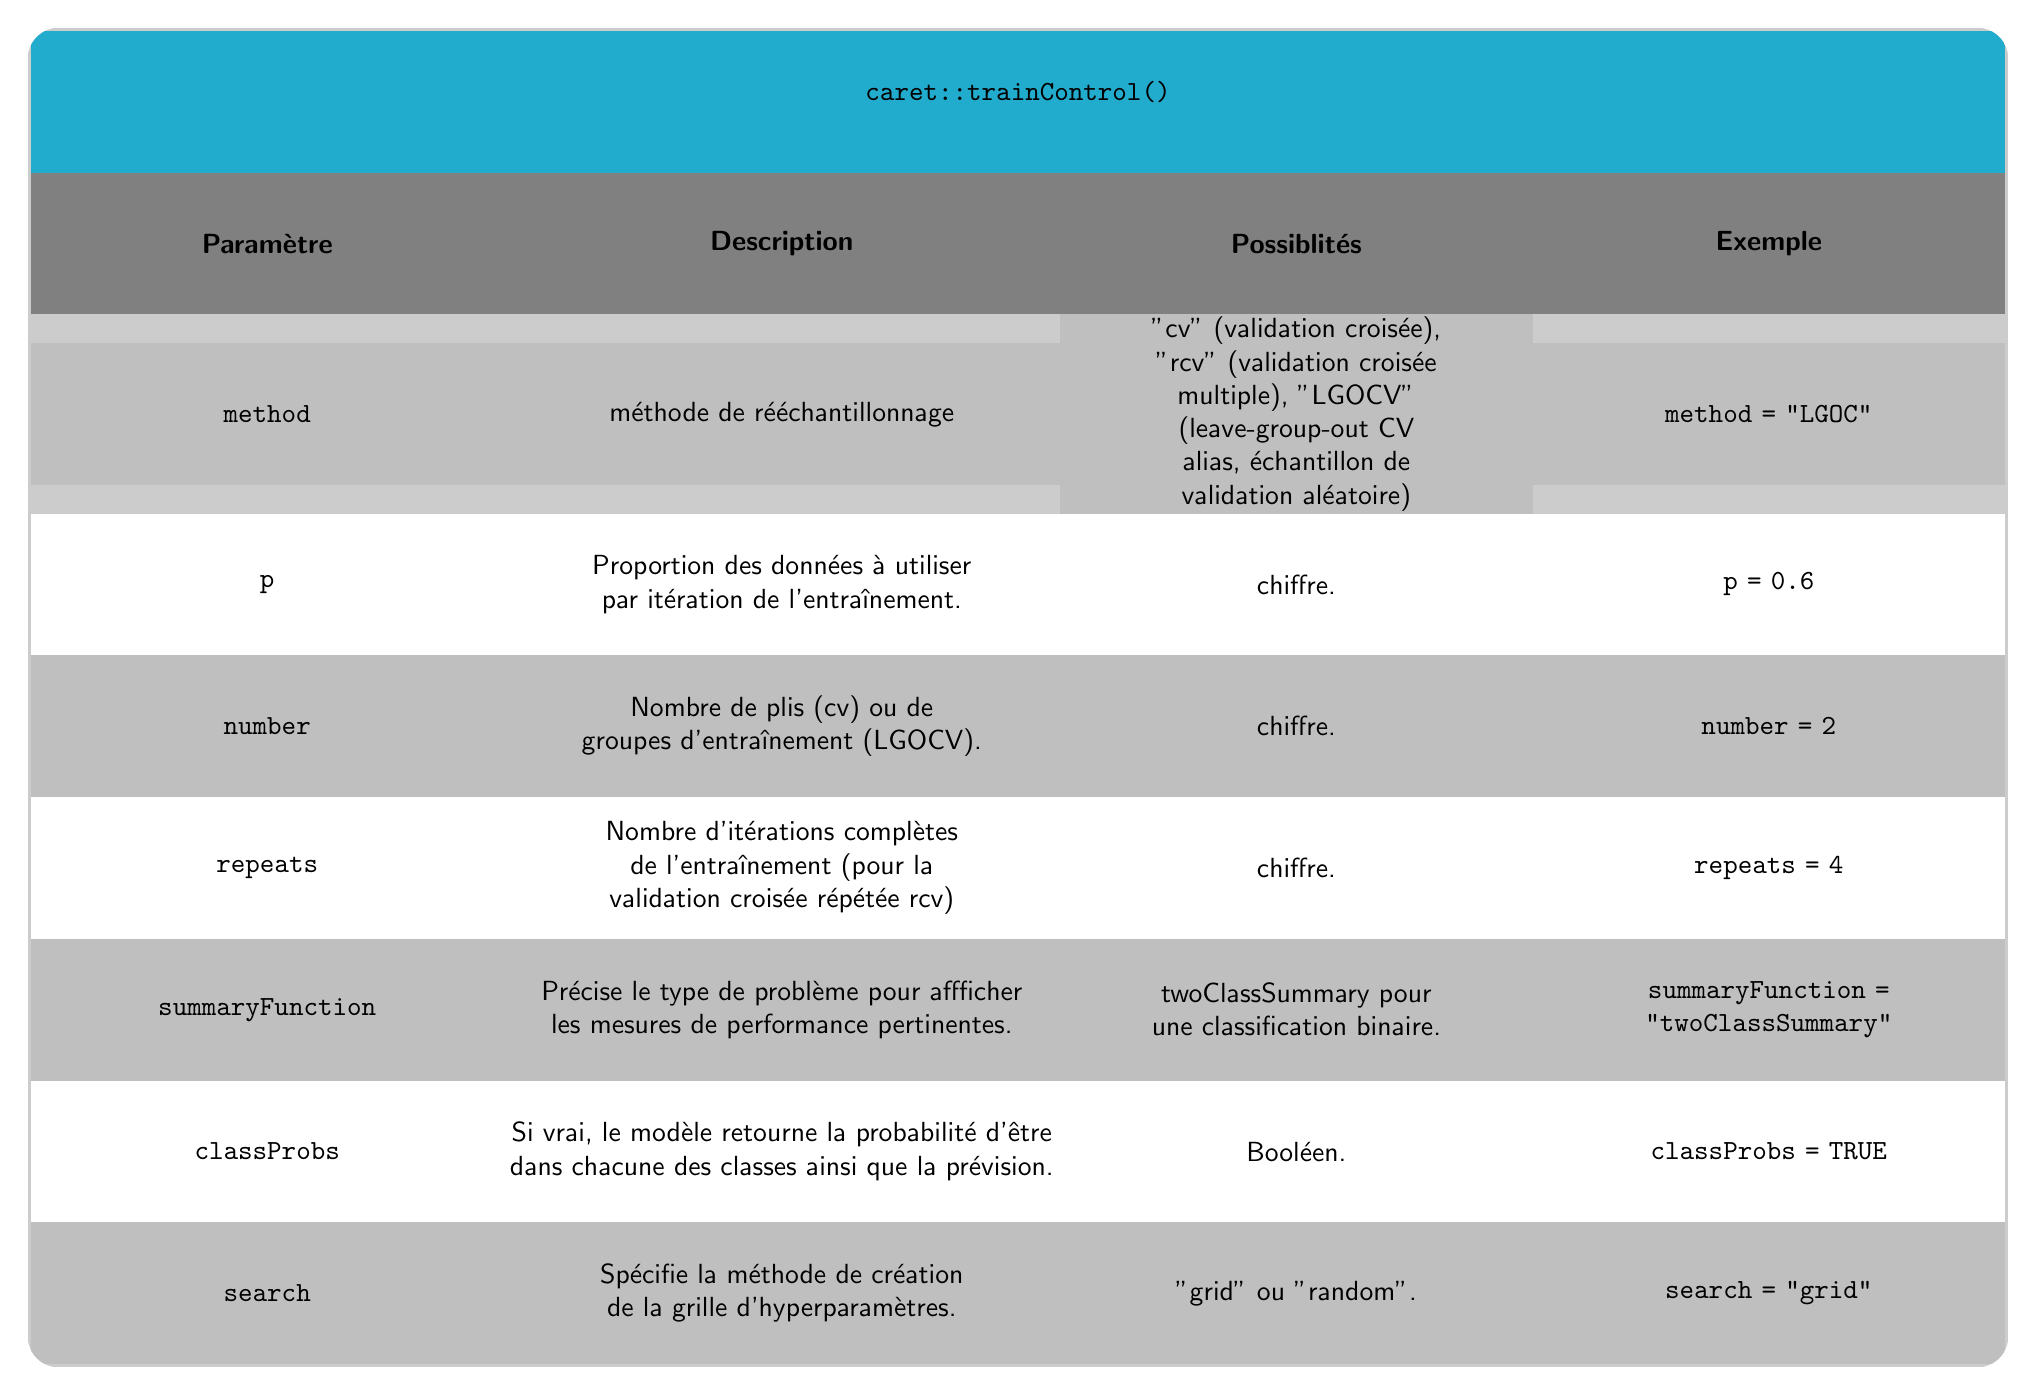
\begin{tikzpicture}
\clip node (m) [
	matrix,
	matrix of nodes,
	fill = black!20, % alternating rows color
	inner sep = 1pt, % width of exterior line
	nodes in empty cells,
	nodes = {
		minimum height = 1.8cm,
		minimum width = 6cm,
		anchor = center,
		outer sep = 0,
		font = \sffamily
	},
	row 1/.style = {
		nodes = {
			fill = ballblue,  % header colour
			text = white,
			font = \bfseries
		}
	},
	column 1/.style = {
		text width = 3cm, 
		align = center,
		nodes = {
			fill = lightgray
		},
		every even row/.style = {
			nodes = {
				fill = white
			}
		}
	},
	column 2/.style = {
		text width = 7cm, 
		align = center,
		nodes = {
			fill = lightgray
		},
		every even row/.style = {
			nodes = {
				fill = white
			}
		}
	},
	column 3/.style = {
		text width = 4cm, 
		align = center,
		nodes = {
			fill = lightgray
		},
		every even row/.style = {
			nodes = {
				fill = white
			}
		}
	},
	column 4/.style = {
		text width = 5cm, 
		align = center,
		nodes = {
			fill = lightgray
		},
		every even row/.style = {
			nodes = {
				fill = white
			}
		}
	},
	row 2 column 1/.style = {nodes = {fill = gray}},
	row 2 column 2/.style = {nodes = {fill = gray}},
	row 2 column 3/.style = {nodes = {fill = gray}},
	row 2 column 4/.style = {nodes = {fill = gray}},
	prefix after command = {
		[rounded corners = 4mm] (m.north east) rectangle (m.south west)
	}
] {
			&			&			&			\\
	\textbf{Paramètre}	&	\textbf{Description}	&	\textbf{Possiblités}	&	\textbf{Exemple} \\
	\texttt{method}	&	méthode de rééchantillonnage	&	"cv" (validation croisée), "rcv" (validation croisée multiple), "LGOCV" (leave-group-out CV alias, échantillon de validation aléatoire) 	&	 \texttt{method = "LGOC"}	\\
	\texttt{p}	&	Proportion des données à utiliser par itération de l'entraînement.	&	chiffre. 	&	 \texttt{p = 0.6}	\\
	\texttt{number}	&	Nombre de plis (cv) ou de groupes d'entraînement (LGOCV).	&	chiffre. 	&	 \texttt{number = 2}	\\
	\texttt{repeats}	&	Nombre d'itérations complètes de l'entraînement (pour la validation croisée répétée rcv)	&	chiffre. 	&	 \texttt{repeats = 4}	\\
	\texttt{summaryFunction}	&	Précise le type de problème pour affficher les mesures de performance pertinentes.	&	twoClassSummary pour une classification binaire. 	&	\texttt{summaryFunction = "twoClassSummary"} 	\\
	\texttt{classProbs}	&	Si vrai, le modèle retourne la probabilité d'être dans chacune des classes ainsi que la prévision.	&	Booléen. 	&	\texttt{classProbs = TRUE} 	\\
	\texttt{search}	&	Spécifie la méthode de création de la grille d'hyperparamètres.	&	"grid" ou "random". 	&	\texttt{search = "grid"} 	\\
};
    \node[fit=(m-1-1)(m-1-4)]{\texttt{caret::trainControl()}};
\end{tikzpicture}

\pagebreak

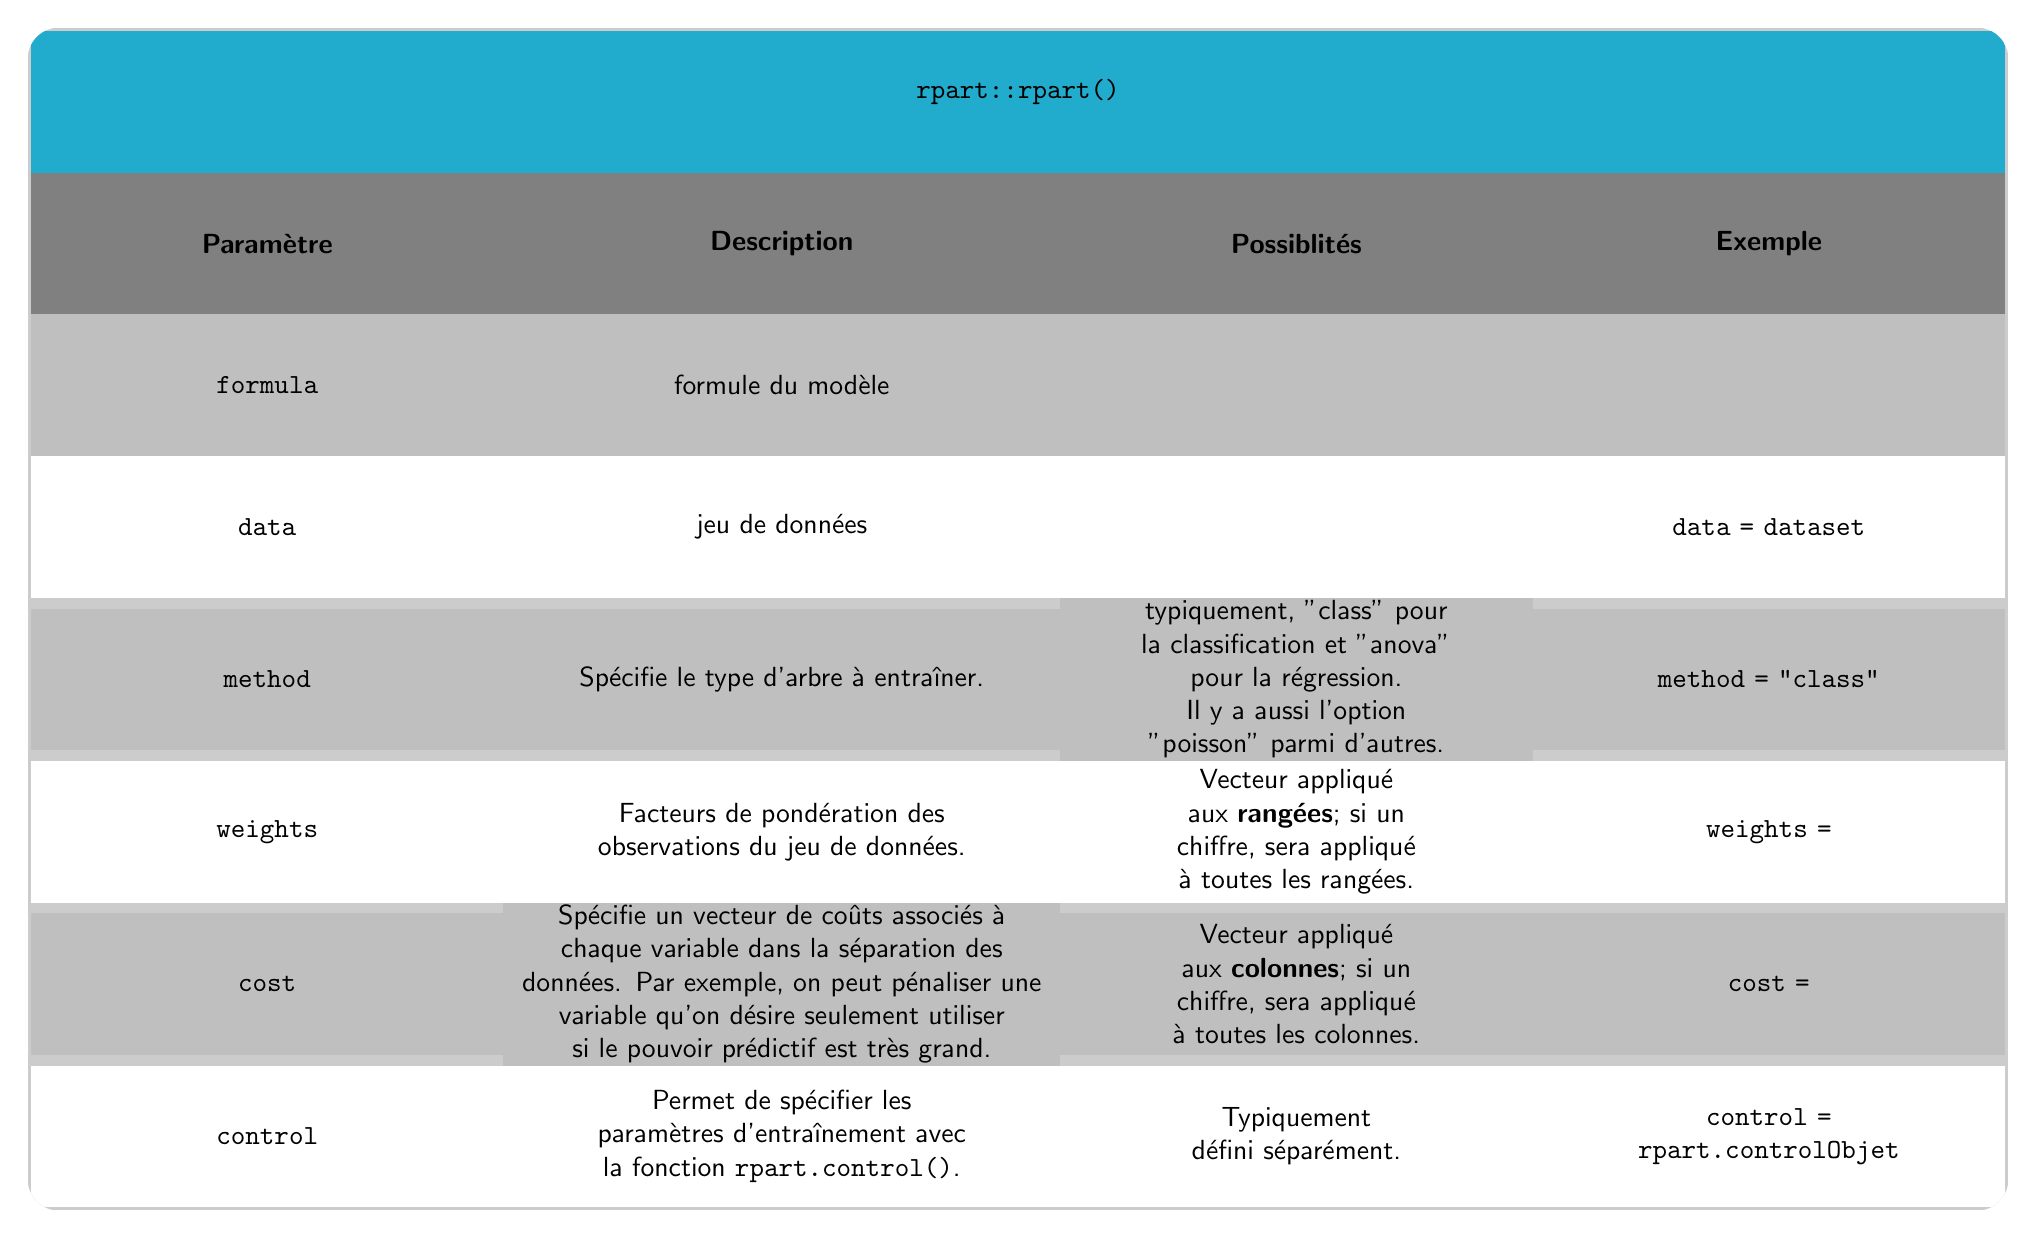
\begin{tikzpicture}
\clip node (m) [
	matrix,
	matrix of nodes,
	fill = black!20, % alternating rows color
	inner sep = 1pt, % width of exterior line
	nodes in empty cells,
	nodes = {
		minimum height = 1.8cm,
		minimum width = 6cm,
		anchor = center,
		outer sep = 0,
		font = \sffamily
	},
	row 1/.style = {
		nodes = {
			fill = ballblue,  % header colour
			text = white,
			font = \bfseries
		}
	},
	column 1/.style = {
		text width = 3cm, 
		align = center,
		nodes = {
			fill = lightgray
		},
		every even row/.style = {
			nodes = {
				fill = white
			}
		}
	},
	column 2/.style = {
		text width = 7cm, 
		align = center,
		nodes = {
			fill = lightgray
		},
		every even row/.style = {
			nodes = {
				fill = white
			}
		}
	},
	column 3/.style = {
		text width = 4cm, 
		align = center,
		nodes = {
			fill = lightgray
		},
		every even row/.style = {
			nodes = {
				fill = white
			}
		}
	},
	column 4/.style = {
		text width = 5cm, 
		align = center,
		nodes = {
			fill = lightgray
		},
		every even row/.style = {
			nodes = {
				fill = white
			}
		}
	},
	row 2 column 1/.style = {nodes = {fill = gray}},
	row 2 column 2/.style = {nodes = {fill = gray}},
	row 2 column 3/.style = {nodes = {fill = gray}},
	row 2 column 4/.style = {nodes = {fill = gray}},
	prefix after command = {
		[rounded corners = 4mm] (m.north east) rectangle (m.south west)
	}
] {
			&			&			&			\\
	\textbf{Paramètre}	&	\textbf{Description}	&	\textbf{Possiblités}	&	\textbf{Exemple} \\
	\texttt{formula}	&	formule du modèle	&	 	&	 	\\
	\texttt{data}	&	jeu de données	&		&	\texttt{data = dataset}	 \\
	\texttt{method}	&	Spécifie le type d'arbre à entraîner.	&	typiquement, "class" pour la classification et "anova" pour la régression. Il y a aussi l'option "poisson" parmi d'autres. 	&	 \texttt{method = "class"}	\\
	\texttt{weights}	&	Facteurs de pondération des observations du jeu de données.	&	Vecteur appliqué aux \textbf{rangées}; si un chiffre, sera appliqué à toutes les rangées. 	&	 \texttt{weights = }	\\
	\texttt{cost}	&	Spécifie un vecteur de coûts associés à chaque variable dans la séparation des données. Par exemple, on peut pénaliser une variable qu'on désire seulement utiliser si le pouvoir prédictif est très grand.	&	Vecteur appliqué aux \textbf{colonnes}; si un chiffre, sera appliqué à toutes les colonnes. 	&	 \texttt{cost = }	\\
	\texttt{control}	&	Permet de spécifier les paramètres d'entraînement avec la fonction \texttt{rpart.control()}.	&	Typiquement défini séparément. 	&	 \texttt{control = rpart.controlObjet}	\\
};
    \node[fit=(m-1-1)(m-1-4)]{\texttt{rpart::rpart()}\addcontentsline{toc}{subsection}{CART}};
\end{tikzpicture}

\pagebreak

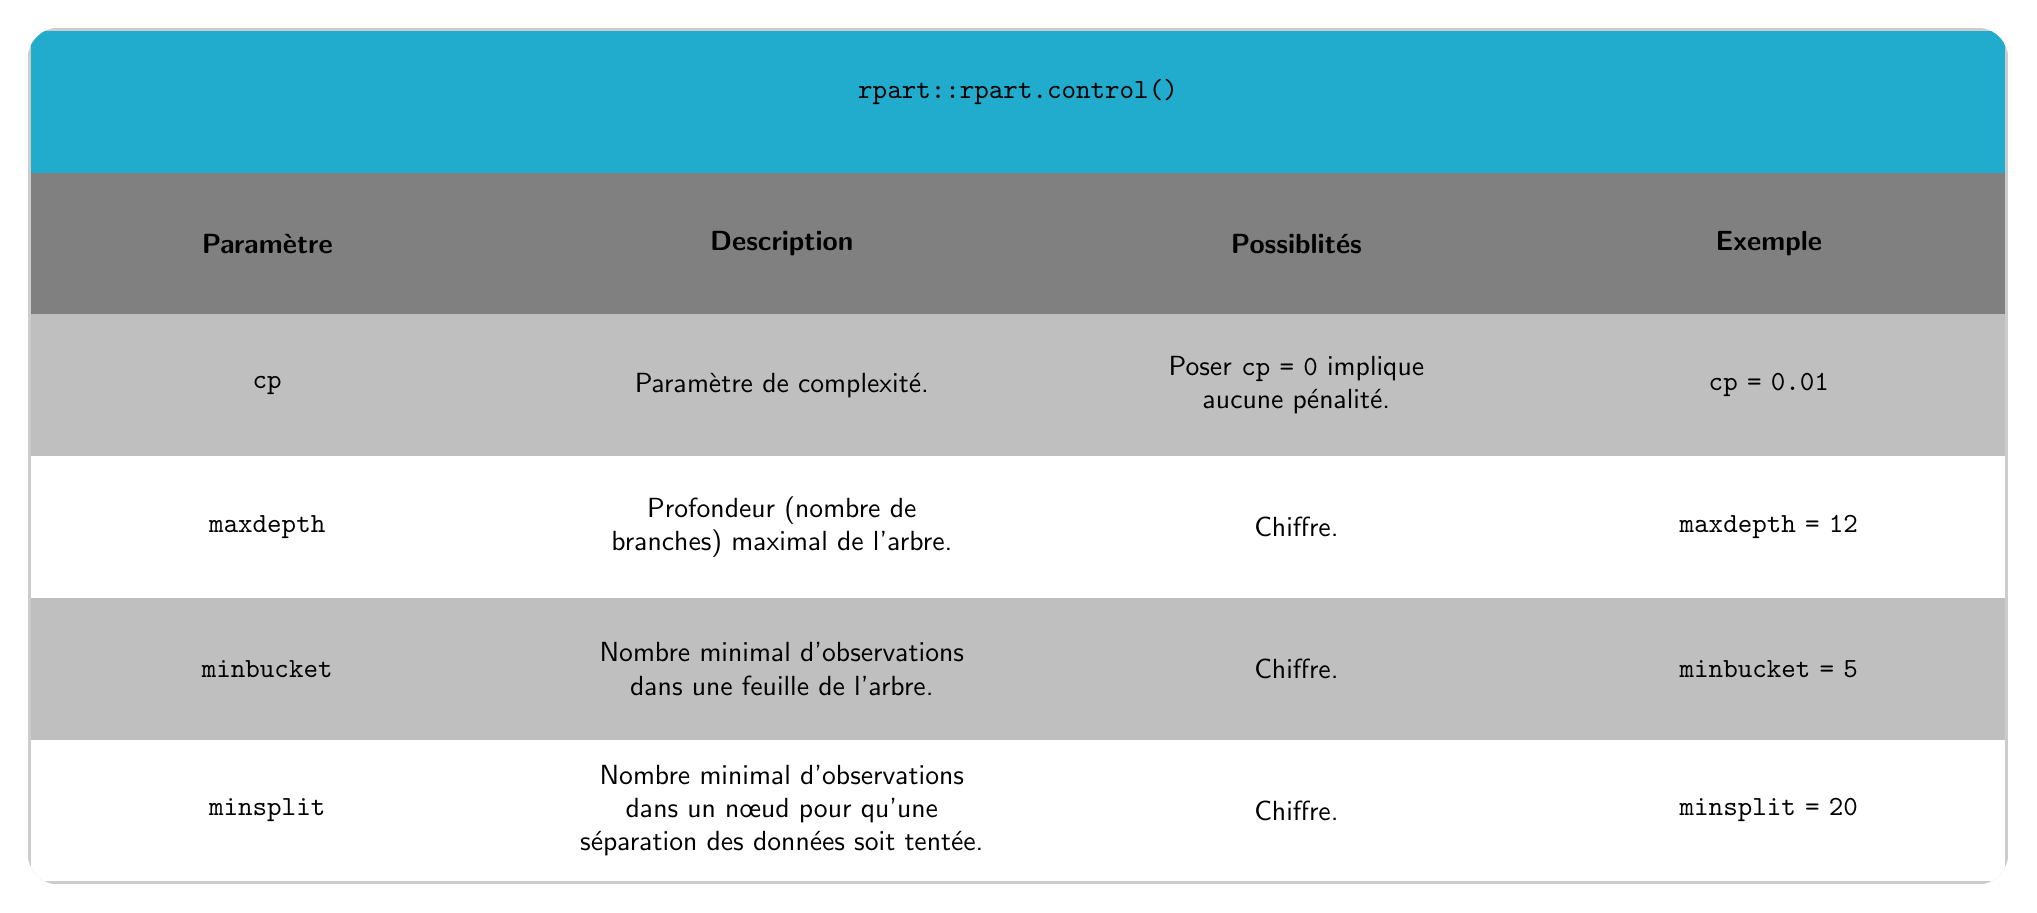
\begin{tikzpicture}
\clip node (m) [
	matrix,
	matrix of nodes,
	fill = black!20, % alternating rows color
	inner sep = 1pt, % width of exterior line
	nodes in empty cells,
	nodes = {
		minimum height = 1.8cm,
		minimum width = 6cm,
		anchor = center,
		outer sep = 0,
		font = \sffamily
	},
	row 1/.style = {
		nodes = {
			fill = ballblue,  % header colour
			text = white,
			font = \bfseries
		}
	},
	column 1/.style = {
		text width = 3cm, 
		align = center,
		nodes = {
			fill = lightgray
		},
		every even row/.style = {
			nodes = {
				fill = white
			}
		}
	},
	column 2/.style = {
		text width = 7cm, 
		align = center,
		nodes = {
			fill = lightgray
		},
		every even row/.style = {
			nodes = {
				fill = white
			}
		}
	},
	column 3/.style = {
		text width = 4cm, 
		align = center,
		nodes = {
			fill = lightgray
		},
		every even row/.style = {
			nodes = {
				fill = white
			}
		}
	},
	column 4/.style = {
		text width = 5cm, 
		align = center,
		nodes = {
			fill = lightgray
		},
		every even row/.style = {
			nodes = {
				fill = white
			}
		}
	},
	row 2 column 1/.style = {nodes = {fill = gray}},
	row 2 column 2/.style = {nodes = {fill = gray}},
	row 2 column 3/.style = {nodes = {fill = gray}},
	row 2 column 4/.style = {nodes = {fill = gray}},
	prefix after command = {
		[rounded corners = 4mm] (m.north east) rectangle (m.south west)
	}
] {
			&			&			&			\\
	\textbf{Paramètre}	&	\textbf{Description}	&	\textbf{Possiblités}	&	\textbf{Exemple} \\
	\texttt{cp}	&	Paramètre de complexité.	&	Poser \texttt{cp = 0} implique aucune pénalité. 	&	 \texttt{cp = 0.01}	\\
	\texttt{maxdepth}	&	Profondeur (nombre de branches) maximal de l'arbre.	&	Chiffre. 	&	 \texttt{maxdepth = 12}	\\
	\texttt{minbucket}	&	Nombre minimal d'observations dans une feuille de l'arbre.	&	Chiffre. 	&	 \texttt{minbucket = 5}	\\
	\texttt{minsplit}	&	Nombre minimal d'observations dans un nœud pour qu'une séparation des données soit tentée.	&	Chiffre. 	&	 \texttt{minsplit = 20}	\\
};
    \node[fit=(m-1-1)(m-1-4)]{\texttt{rpart::rpart.control()}};
\end{tikzpicture}

\pagebreak

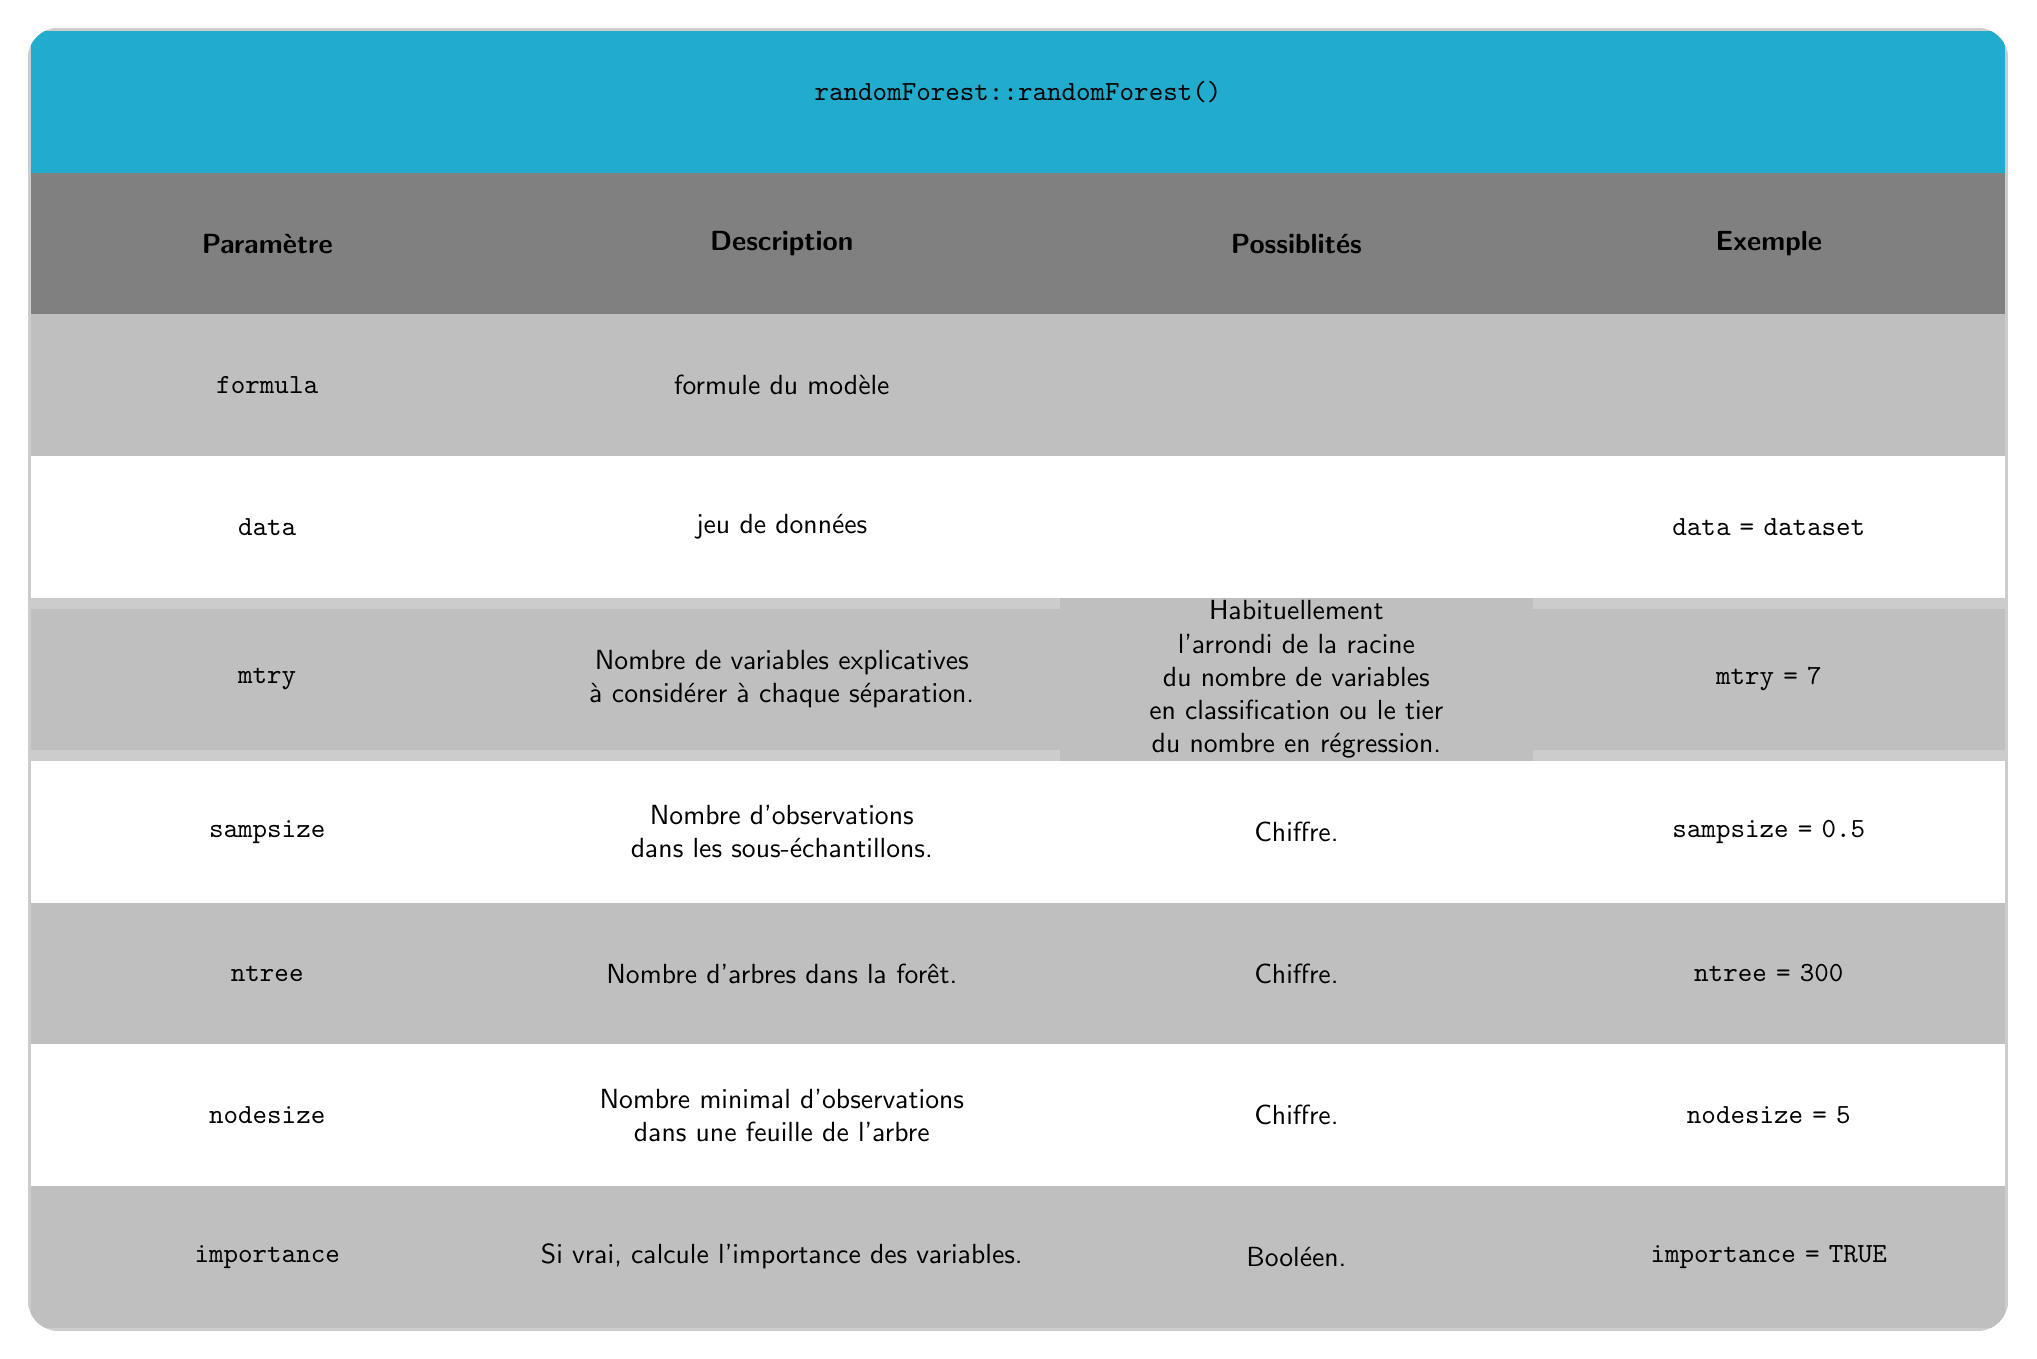
\begin{tikzpicture}
\clip node (m) [
	matrix,
	matrix of nodes,
	fill = black!20, % alternating rows color
	inner sep = 1pt, % width of exterior line
	nodes in empty cells,
	nodes = {
		minimum height = 1.8cm,
		minimum width = 6cm,
		anchor = center,
		outer sep = 0,
		font = \sffamily
	},
	row 1/.style = {
		nodes = {
			fill = ballblue,  % header colour
			text = white,
			font = \bfseries
		}
	},
	column 1/.style = {
		text width = 3cm, 
		align = center,
		nodes = {
			fill = lightgray
		},
		every even row/.style = {
			nodes = {
				fill = white
			}
		}
	},
	column 2/.style = {
		text width = 7cm, 
		align = center,
		nodes = {
			fill = lightgray
		},
		every even row/.style = {
			nodes = {
				fill = white
			}
		}
	},
	column 3/.style = {
		text width = 4cm, 
		align = center,
		nodes = {
			fill = lightgray
		},
		every even row/.style = {
			nodes = {
				fill = white
			}
		}
	},
	column 4/.style = {
		text width = 5cm, 
		align = center,
		nodes = {
			fill = lightgray
		},
		every even row/.style = {
			nodes = {
				fill = white
			}
		}
	},
	row 2 column 1/.style = {nodes = {fill = gray}},
	row 2 column 2/.style = {nodes = {fill = gray}},
	row 2 column 3/.style = {nodes = {fill = gray}},
	row 2 column 4/.style = {nodes = {fill = gray}},
	prefix after command = {
		[rounded corners = 4mm] (m.north east) rectangle (m.south west)
	}
] {
			&			&			&			\\
	\textbf{Paramètre}	&	\textbf{Description}	&	\textbf{Possiblités}	&	\textbf{Exemple} \\
	\texttt{formula}		&	formule du modèle	&	 	&	 	\\
	\texttt{data}		&	jeu de données	&		&	\texttt{data = dataset}	 \\
	\texttt{mtry}		&	Nombre de variables explicatives à considérer à chaque séparation.	&	Habituellement l'arrondi de la racine du nombre de variables en classification ou le tier du nombre en régression. 	&	\texttt{mtry = 7}	\\
	\texttt{sampsize}	&	Nombre d'observations dans les sous-échantillons.	&	Chiffre.  	&	\texttt{sampsize = 0.5}	\\
	\texttt{ntree}		&	Nombre d'arbres dans la forêt.	&	Chiffre. 	&	\texttt{ntree = 300}	\\
	\texttt{nodesize}	&	Nombre minimal d'observations dans une feuille de l'arbre 	&	 Chiffre.	&	\texttt{nodesize = 5}	\\
	\texttt{importance}	&	Si vrai, calcule l'importance des variables.	&	Booléen. 	&	\texttt{importance = TRUE} 	\\
};
    \node[fit=(m-1-1)(m-1-4)]{\texttt{randomForest::randomForest()}\addcontentsline{toc}{subsection}{Forêt Aléatoire}};
\end{tikzpicture}

\pagebreak

\begin{description}
	\item[\texttt{mod.iml $\leftarrow$ Predictor\$new(modeleTrain)} puis \texttt{FeatureImp\$new(mod.iml, loss = "METRIC", compare = "difference",  n.repetitions = 5)}]		Importance des variables selon l'erreur de classification "METRIC" (e.g., "mse") que l'on peut ensuite visualiser.
	\item[\texttt{FeatureEffect\$new(mod.iml, "variable1", method = "pdp", grid.size = X)}]	Graphique de dépendance partielle univariée (PDP).
	\item[\texttt{FeatureEffect\$new(mod.iml, feature = c("variable1", "variable2"), method = "pdp", grid.size = X)}]	Graphique de dépendance partielle bivariée (PDP).
	\item[NOTE]	Si l'on remplace \texttt{method = "pdp"} par \texttt{method = "ice"} on obtient un graphique d'espérance conditionnelle individuelle (ICE).
	\item[\texttt{Interaction\$new(mod.iml, "variableImp")}]	Statistique H de Friedman pour quantifier les interactions entre la variable la plus importante et les autres.
\end{description}

\end{document}
